
%\usepackage{graphicx}
%\usepackage{caption}
%\usepackage{subcaption}

%\usepackage{amsthm}
%\usepackage{amssymb}
%\usepackage{amsmath}

%\usepackage{algpseudocode}
%\usepackage{algorithm}
%\usepackage{algorithmicx}

%\theoremstyle{theorem}
%\newtheorem{theorem}{Теорема}
%%\newtheorem{coroll}{Следствие}[theorem]
\theoremstyle{definition}
\newtheorem{defn}{Определение}
\theoremstyle{proposition}
\newtheorem{prop}{Предложение}

\title{Синтаксический анализ данных, представленных в виде контекстно-свободной грамматики}

\titlerunning{Синтаксический анализ контекстно-свободных грамматик}

\author{Ковалев Дмитрий Александрович}

\authorrunning{Д. А. Ковалев}

\tocauthor{Д. А. Ковалев}
\institute{Санкт-Петербургский государственный университет\\
\email{lares77@yandex.ru}}


\maketitle

\begin{abstract}
Многие программы в процессе работы формируют из строк исходный код на некотором языке программирования и передают его для исполнения в соответствующее окружение (пример --- dynamic SQL). Для статической проверки корректности динамически формируемого выражения используются различные методы, одним из которых является синтаксический анализ регулярной аппроксимации множества значений такого выражения. Аппроксимация может содержать строки, не принадлежащие исходному множеству значений, в том числе синтаксически некорректные. Анализатор в данном случае сообщит об ошибках, которые на самом деле отсутствуют в выражении, генерируемом программой. В докладе будет описан алгоритм синтаксического анализа более точной, чем регулярная, контекстно-свободной аппроксимации динамически формируемого выражения.
\end{abstract}

\section{Введение}

Большая часть современного программного обеспечения написана на языках, позволяющих  динамически выделять память, таких как \texttt{C++}, \texttt{Java}, \texttt{C\#}. Автоматический анализ программ на таких языках является трудоёмкой задачей~\cite{distefano2009attacking}. При этом даже корректные с теоретической точки зрения методы анализа могут оказаться неэффективными на реальных индустриальных проектах из-за их размеров~\cite{calcagno2011compositional}. Для решения проблемы масштабирования анализа на большие проекты были предложены различные \emph{композициональные} техники анализа программ, которые хорошо зарекомендовали себя на практике~\cite{gurfinkel2015seahorn,anand2008demand,distefano2008jstar,calcagno2011infer}. Такие техники подразумевают анализ функций в \emph{изоляции}, то есть вне контекста конкретного вызова, и переиспользование артефактов анализа. Таким образом можно свести верификацию больших систем к задаче верификации набора небольших фрагментов кода.

Идея композиционального анализа представляется вполне естественной ввиду модульной природы программного обеспечения. Однако большинство существующих композициональных техник являются \emph{неточными} в том смысле, что они аппроксимируют снизу или сверху пространства состояний программы. Типичная аппроксимирующая снизу техника может заключаться в конечной раскрутке циклов и рекурсии или исполнении некоторых функций на конкретных значениях, например~\cite{tillmann2008pex}. Аппроксимирующие сверху техники, такие как абстрактная интерпретация~\cite{cousot1977abstract}, как правило работают в абстрактном домене. Простым примером такого домена может быть $\{+, -, 0\}$ для анализа программ с целыми числами. Анализатор с этим доменом будет интерпретировать инструкцию \lstinline{x := 42} как \lstinline{x := +}, что позволит рассуждать о знаках переменных, но не о их точных значениях.

В данной работе представлен формализм, позволяющий проводить \emph{точный} композициональный анализ программ с динамической памятью. Он основывается на концепции \emph{композициональной символьной памяти}. На базе указанного формализма строится подход к модульной верификации императивных программ с динамической памятью, функциями высшего порядка и неограниченной рекурсией. Совмещение композициональной символьной памяти и широко известной техники композиционального символьного исполнения~\cite{godefroid2007compositional} позволяет построить инструмент точного модульного анализа.

Композициональная символьная память является расширением классической модели символьной памяти. Расширение заключается в том, что значения в \emph{символьных кучах} могут представляться \ruquote{ленивыми} \emph{ячейками}, аналогично методам ленивого инстанцирования~\cite{khurshid2003generalized}. Содержимое такой ячейки~--- источник символьного значения~--- может быть символьным выражением над другими ячейками, что позволяет кодировать поведение функций, работающих с произвольными рекурсивными типами данных. В данной работе представлена формальная модель композициональной символьной памяти и доказаны некоторые свойства, показывающие её применимость.

Также в работе представлено исчисление, обобщающее концепцию символьных куч. Главное достоинство этого исчисления в том, что оно даёт возможность символьно исполнять императивные программы с динамической памятью без раскрутки циклов и рекурсивных функций, позволяя избежать проблемы взрыва путей исполнения. Предлагаемое исчисление позволяет алгоритму символьного исполнения \emph{точно} описать все поведения функции, породив некоторый набор \emph{уравнений на состояния}.

Решение таких уравнений требует использования достаточно мощного инструмента логических рассуждений и синтеза индуктивных инвариантов. Вместо принятых в символьном исполнении SMT-решателей, предлагается использовать \emph{решатели дизъюнктов Хорна с ограничениями} (constrained Horn clauses)~\cite{bjorner2015horn}. Непосредственное кодирование уравнений над состояниями даёт дизъюнкты Хорна \emph{высшего порядка}~\cite{cathcart2017higher}, которые могут быть сведены к дизъюнктам первого порядка при помощи инструментов вывода ограниченных (refinement) типов~\cite{vazou2015bounded,unno2013automating,zhu2013compositional}.

На предлагаемое в данной работе исчисление можно смотреть как на алгоритм построения соответствия между программами с динамической памятью и чистыми функциями второго порядка. В качестве побочного эффекта, этот алгоритм позволяет транслировать произвольные императивные программы с динамической памятью в функциональные языки. Композициональная природа предлагаемого подхода позволяет получать функциональные программы, похожие по структуре на изначальные.

Основные результаты данной работы:
\begin{enumerate}
    \item концепция композициональной символьной памяти;
    \item доказательства её свойств;
    \item понятия \emph{обобщённых символьных куч} и \emph{уравнений на состояния}, исчисление для их построения и упрощения;
    \item алгоритм композиционального символьного исполнения императивных программ с динамической памятью без раскрутки;
    \item сведение уравнений на состояния к дизъюнктам Хорна с ограничениями.
\end{enumerate}

\section{Постановка задачи}
Целью данной работы является разработка алгоритма ослабленного синтаксического 
анализа для регулярной аппроксимации множества значений динамически формируемого
выражения, который для всех корректных относительно некоторой эталонной 
грамматики цепочек строит конечное представление множества деревьев разбора, при
этом цепочки, не принадлежащие эталонному языку, игнорируются.

В рамках данной дипломной работы поставлены следующие задачи.
\begin{itemize}
  \item Разработать алгоритм синтаксического анализа динамически формируемых 
        выражений, поддерживающий работу с произвольными входными графами.
  \item Реализовать предложенный алгоритм.
  \item Доказать корректность алгоритма.
  \item Провести апробацию.
\end{itemize}
\section{Обзор}

В данной работе используется понятие \textit{рекурсивного автомата} \cite{tellier2006ra} --- удобного представления произвольной контекстно-свободной грамматики.
Описание этой абстракции приводится в первом параграфе обзора.

Предлагаемый в работе алгоритм основан на алгоритме синтаксического анализа регулярных множеств, который, в свою очередь, является модификацией алгоритма обобщенного синтаксического анализа Generalized LL (GLL, \cite{gll}).
Об этих алгоритмах и о проекте, в рамках которого проведена разработка предложенного решения, также будет рассказано в обзоре.

\subsection{Рекурсивные автоматы и КС-грамматики}
Введем понятие рекурсивного автомата, которое потребуется для дальнейшего изложения.

\begin{defn}
	Рекурсивный автомат R --- это кортеж $(\Sigma, Q, \delta, q_0, q_f)$, где $\Sigma$ --- конечное множество терминальных символов, $Q$ --- конечное множество состояний автомата, $\delta : Q \times (\Sigma \cup Q) \rightarrow 2^Q$ --- функция переходов, $q_0 \in Q$ --- начальное состояние, $q_f$ --- конечное состояние. 
\end{defn}

Можно заметить, что данное определение практически идентично определению стандартного конечного автомата. 
Единственное отличие состоит в том, что метками на ребрах рекурсивного автомата могут быть как терминальные символы (терминальные переходы), так и состояния (нетерминальные переходы).
Класс рекурсивных автоматов обладает такой же выразительностью, как и контекстно-свободные грамматики, т.е. позволяет описать любой контекстно-свободный язык. 
Более того, грамматика тривиальным образом может быть преобразована в рекурсивный автомат (обратное тоже верно) \cite{tellier2006ra}. 
Пример рекурсивного автомата, построенного по грамматике, можно увидеть на рис. \ref{fig:ra_ex}.

\begin{figure}[h]
	\centering
		$$
		\begin{array}{crcl}
		&S' & ::= & S \\
		&S  & ::= & \texttt{[ } S \texttt{ ]}\\
		&S  & ::= & \mbox{\texttt{a}}
		\end{array}
		$$
		\caption{Грамматика $G_1$}
\end{figure}
\begin{figure}[h]
	\centering
		\centering
		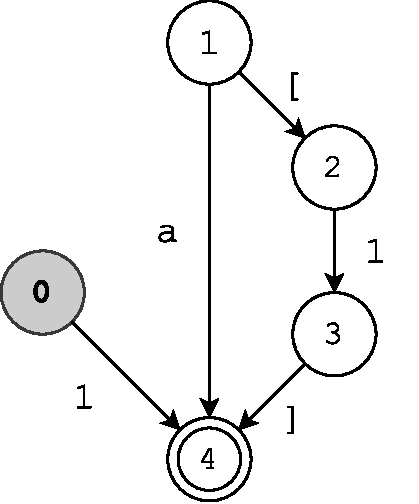
\includegraphics[width=4cm]{Kovalev/pictures/ra_example.pdf}
		\caption{Рекурсивный автомат для $G_1$}
	\caption{КС-грамматика и эквивалентный ей рекурсивный автомат}
	\label{fig:ra_ex}
\end{figure}

\subsection{GLL-алгоритм и его модификации}

Классические алгоритмы нисходящего и восходящего синтаксического анализа предполагают использование грамматики, которая является в достаточной мере однозначной. 
В противном случае, управляющие таблицы анализаторов содержат конфликты, из-за чего нельзя гарантировать корректное поведение на любых входных данных. 
Для работы с сильно неоднозначными грамматиками используются алгоритмы \textit{обобщенного синтаксического анализа}, которые позволяют рассмотреть все возможные пути разбора строки и построить соответствующие деревья вывода.
Поиск шаблонов не требует наличия деревьев вывода, поэтому в дальнейшем алгоритмы синтаксического анализа рассматриваются только как механизм, позволяющий определить принадлежность строки языку.

\subsubsection{Оригинальный GLL-алгоритм}

Generalized LL (GLL) --- алгоритм, обобщающий идеи нисходящего синтаксического анализа. GLL, в отличие от стандартных алгоритмов LL-класса, позволяет использовать для анализа произвольную контекстно-свободную грамматику, в том числе содержащую леворекурсивные правила. Вместе с тем, GLL наследует такие полезные свойства алгоритмов нисходящего анализа, как непосредственную связь с грамматикой и простоту отладки и диагностики ошибок.

Для обработки неоднозначностей GLL разделяет стек анализатора на несколько ветвей, каждая из которых соответствует возможному пути разбора. При таком подходе необходимо компактное представление множества стеков, в качестве которого выступает Graph Structured Stack (GSS). В работе \cite{Afroozeh2015gss} была представлена модификация GSS, которая позволяет увеличить эффективность GLL-анализа. Вершины такого представления хранят в себе номер нетерминала и позицию в строке, с которой начался разбор подстроки, соответствующей ему. На ребрах хранятся позиции в грамматике (вида $X \rightarrow \alpha A \cdot \beta$), на которые необходимо вернуться после завершения разбора нетерминала. 
%При помощи GSS также решается проблема бесконечного роста стеков при обработке левой рекурсии: при попытке создать вершину, которая уже существует, в граф добавится

Основной идеей GLL является использование \textit{дескрипторов}, позволяющих полностью описывать состояние анализатора в текущий момент времени.

\begin{defn}
	Дескриптор --- это тройка (L, u, i), где:
	\begin{itemize}
		\setlength\itemsep{0em}
		\item L --- текущая позиция в грамматике вида $A \rightarrow \alpha \cdot \beta$;
		\item u --- текущая вершина GSS;
		\item i --- позиция во входном потоке.
	\end{itemize}
\end{defn}  

В процессе работы поддерживается глобальная очередь дескрипторов. В начале каждого шага исполнения алгоритм берет следующий в очереди дескриптор и производит действия в зависимости от позиции в грамматике и текущего входного символа, передвигая соответствующие указатели. 
При наличии конфликтов в грамматике алгоритм добавляет дескрипторы для каждого возможного пути анализа в конец очереди.

\subsubsection{Поддержка грамматик в EBNF}

В работе \cite{Gorokhov2017ebnf} была описана модификация GLL, которая позволяет использовать грамматики, записанные в расширенной форме Бэкуса-Наура (EBNF). Грамматика такого вида трансформируется в соответствующий рекурсивный автомат, в котором затем минимизируется количество состояний. Синтаксический анализ производится без построения управляющих таблиц: алгоритм обходит рекурсивный автомат в соответствии со входным потоком символов. При обработке текущего дескриптора $(C_S, C_U, i)$, где $C_S$ --- вершина автомата (эквивалент позиции в грамматике), $C_U$ --- вершина GSS, $i$ --- позиция в строке, могут возникать следующие ситуации.

\begin{itemize}
	\item $C_S$ --- финальное состояние. Показывает, что разбор текущего нетерминала завершен. Необходимо осуществить возврат из $C_U$ по меткам на исходящих из нее ребрах.
	\item Присутствует нетерминальный переход из $C_S$. В данном случае необходимо начать разбор указанного нетерминала $X$. Для этого в GSS должна быть создана новая вершина $(X, i)$, если таковой не было ранее, а текущая вершина автомата изменена на стартовую для $X$.
	\item Присутствует терминальный переход из $C_S$. Необходимо сравнить терминал на ребре автомата с текущим входным символом. Если они совпадают, то осуществить переход в вершину автомата, на которую указывает ребро, и передвинуть указатель в строке.
\end{itemize}

За счет уменьшения количества состояний в автомате удается достичь прироста в производительности по сравнению со стандартным GLL-алгоритмом.

\subsubsection{Синтаксический анализ графов}

Стандартными входными данными для алгоритмов синтаксического анализа являются линейные последовательности токенов. На основе GLL был разработан алгоритм, который позволяет производить синтаксический анализ регулярных множеств строк, представленных в виде конечного автомата (который, в свою очередь, является ориентированным графом с токенами на ребрах).

Поддержка нелинейного входа не потребовала существенных изменений в оригинальном алгоритме. Дескрипторы модифицированного алгоритма хранят номер вершины входного графа вместо позиции в строке. Также, на шаге исполнения просматривается не единственный текущий символ, а множество символов на ребрах, исходящих из текущей вершины.

Производительность данного алгоритма, как и обычного GLL, может быть увеличена при помощи представления входной грамматики в виде рекурсивного автомата. В таком случае, алгоритм будет производить обход двух автоматов --- рекурсивного и конечного. Ситуации, возникающие при обработке дескрипторов, не отличаются от описанных ранее ситуаций для линейного входа. Псевдокод данной модификации приведен в приложении. Рассматривается вариант без построения деревьев вывода, алгоритм возвращает длины корректных цепочек, порождаемых автоматом. 

\subsection{Проект YaccConstructor}

YaccConstructor \cite{SemyonPhD} --- исследовательский проект лаборатории языковых инструментов JetBrains на математико-механическом факультете СПбГУ, направленный на исследования в области лексического и синтаксического анализа. Проект включает в себя одноименную модульную платформу для разработки лексических и синтаксических анализаторов, содержащую большое количество компонент: язык описания грамматик YARD \cite{yard_url}, преобразования над грамматиками и др. Основным языком разработки является F$\#$.

Ранее в рамках YaccConstructor были реализованы генераторы GLL-анализаторов, описание которых было приведено в данном обзоре. 

\section{Разрешимость задачи синтаксического \\ анализа контекстно-свободного представления}
Как было сказано ранее, задачу поиска шаблона, при условии, что и шаблон, и данные, в которых осуществляется поиск, представлены контекстно-свободными грамматиками, мы назовем синтаксическим анализом контекстно-свободного представления. В данном разделе определяются ограничения, при которых подобная задача разрешима.

Для доказательства предложений, сформулированных далее, используется следующая теорема \cite{Nederhof}.

\begin{theorem}[Nederhof, Satta]
	Пусть $G_1$ --- произвольная контекстно-свободная грамматика, $G_2$ --- грамматика, которая не содержит непосредственной или скрытой рекурсии. Тогда проблема проверки пустоты пересечения языков, порождаемых данными грамматиками, относится к классу PSPACE-complete.
\end{theorem}

Рассмотрим случай, когда грамматика данных задает ровно одну строку. Пусть $G_t$ --- произвольная КС-грамматика, задающая шаблоны для поиска, а $G_d$ --- КС-грамматика, которая не содержит непосредственной или скрытой рекурсии. $L(G_t)$ и $L(G_d)$ --- языки, порождаемые грамматиками, при этом $L(G_d) = \{\omega\}$, где $\omega$ --- исходные данные, к которым был применен алгоритм сжатия. 
Необходимо определить, существуют ли такие строки $\omega'$, что $\omega' \in L(G_t)$ и $\omega'$ --- подстрока $\omega$. 

\begin{prop}
	При выполнении описанных условий задача синтаксического анализа КС-представления разрешима.
\end{prop}

\begin{proof}
Пользуясь эквивалентностью представлений, можно записать грамматику $G_d$ в виде рекурсивного автомата $R_d$. Рассмотрим рекурсивный автомат $R_{i,\,j}$, полученный из $R_d$ путем замены стартового состояния на $i \in Q(R_d)$ и назначения терминирующего (финального, из которого не могут быть совершены переходы) состояния $j \in Q(R_d)$. Такой автомат описывает грамматику, которая является представлением некоторой подстроки $\omega$. 
Рассмотрев все возможные пары $i$ и $j$, получаем конечное множество грамматик, для каждой из которых необходимо проверить, содержится ли строка, порождаемая ей, в языке $L(G_t)$. 
Согласно теореме 1, такая проверка является разрешимой задачей и принадлежит к классу PSPACE-complete.
\end{proof}

Отдельно отметим, что для описанных процедур используется лишь исходный автомат, эквивалентный грамматике $G_d$. 
Условия задачи поиска шаблонов непосредственно в контекстно-свободном представлении, таким образом, выполняются. 
Верна также разрешимость более общей задачи.

\begin{prop}
	Пусть грамматика $G_d$ задает конечное множество строк $L(G_d) = \{\omega_1, \, \dots \, , \omega_n \}$. Необходимо определить, существуют ли строки $\omega'$, для которых верно: $\omega' \in L(G_t)$ и $\omega'$ --- подстрока одной из строк $\omega_i \in L(G_d)$. Данная задача разрешима и принадлежит классу PSPACE-complete.
\end{prop}

\begin{proof}
	Как и в предыдущем доказательстве, используем запись грамматики в виде рекурсивного автомата $R_d$ и рассмотрим автоматы $R_{i, j}$. В данном случае каждый из этих автоматов представляет собой грамматику, которая порождает некоторое конечное множество подстрок исходных строк из $L(G_d)$. Проверка пустоты пересечения такой грамматики с $G_t$ также соответствует условиям теоремы 1.
\end{proof}

В случае, когда грамматика $G_d$ представляет собой бесконечный регулярный язык (т.е. содержит левую и/или правую рекурсию), разрешимость задачи поиска шаблонов установить не удается. Подход, использованный ранее в доказательстве предложений, не может быть применен, так как части рекурсивного автомата, представляющего грамматику $G_d$, также могут содержать рекурсивные переходы, что выходит за рамки условия теоремы 1. Проверка разрешимости и определение класса сложности задачи проверки пустоты пересечения произвольной и регулярной КС-грамматик в настоящее время остаются открытыми проблемами \cite{Nederhof}.
\section{An algorithm for CFPQ using relational query semantics}
In this section, we show how the context-free path query evaluation using the relational query semantics can be reduced to the calculation of matrix transitive closure $a^{cf}$, prove the correctness of this reduction, introduce an algorithm for computing the transitive closure $a^{cf}$, and provide a step-by-step demonstration of this algorithm on a small example.

\subsection{Reducing CFPQ to transitive closure} \label{section_reducing}
In this section, we show how the context-free relations $R_A$ can be calculated by computing the matrix transitive closure $a^{cf}$.

We introduce another definition of the transitive closure of an arbitrary square matrix $a$ as $$a^{cf} = a^{(1)} \cup a^{(2)} \cup \cdots$$ where $a^{(1)} = a$ and $a^{(i)} = a^{(i-1)} \cup (a^{(i-1)} \times a^{(i-1)}), ~i \ge 2.$

To show that Valiant's and this definitions of the matrix transitive closure are equivalent, we introduce the partial order $\succeq$ on matrices with the fixed size which have subsets of $N$ as elements. For square matrices $a, b$ of the same size, we denote $a \succeq b$ iff $a_{i,j} \supseteq b_{i,j}$, for every $i, j$. For these two definitions of transitive closure, the following lemmas and theorem hold.

\begin{lemma}\label{lemma:cf_geq_valiant}
	Let $G =(N,\Sigma,P)$ be a grammar, let $a$ be a square matrix. Then $a^{(k)} \succeq a^{(k)}_+$ for any $k \geq 1$.
\end{lemma}
\begin{proof}(Proof by Induction)
	
	\textbf{Basis}: The statement of the lemma holds for $k = 1$, since $$a^{(1)} = a^{(1)}_+ = a.$$
	
	\textbf{Inductive step}: Assume that the statement of the lemma holds for any $k \leq (p - 1)$ and show that it also holds for $k = p$ where $p \geq 2$. For any $i \geq 2$ $$a^{(i)} = a^{(i-1)} \cup (a^{(i-1)} \times a^{(i-1)}) \Rightarrow a^{(i)} \succeq a^{(i-1)}.$$ Hence, by the inductive hypothesis, for any $i \leq (p-1)$ $$a^{(p-1)} \succeq a^{(i)} \succeq a^{(i)}_+.$$ Let $1 \leq j \leq (p - 1)$. The following holds $$(a^{(p-1)} \times a^{(p-1)}) \succeq (a^{(j)}_+ \times a^{(p-j)}_+),$$ since $a^{(p-1)} \succeq a^{(j)}_+$ and $a^{(p-1)} \succeq a^{(p-j)}_+$. By the definition, $$a^{(p)}_+ = \bigcup^{p-1}_{j=1}{a^{(j)}_+ \times a^{(p-j)}_+}$$ and from this it follows that $$(a^{(p-1)} \times a^{(p-1)}) \succeq a^{(p)}_+.$$ By the definition, $$a^{(p)} = a^{(p-1)} \cup (a^{(p-1)} \times a^{(p-1)}) \Rightarrow a^{(p)} \succeq (a^{(p-1)} \times a^{(p-1)}) \succeq a^{(p)}_+$$ and this completes the proof of the lemma.
\end{proof}

\begin{lemma}\label{lemma:valiant_geq_cf}
	Let $G =(N,\Sigma,P)$ be a grammar, let $a$ be a square matrix. Then for any $k \geq 1$ there is $j \geq 1$, such that $(\bigcup^{j}_{i=1}{a^{(i)}_+}) \succeq a^{(k)}$.
\end{lemma}
\begin{proof}(Proof by Induction)
	
	\textbf{Basis}: For $k = 1$ there is $j = 1$, such that $$a^{(1)}_+ = a^{(1)} = a.$$ Thus, the statement of the lemma holds for $k = 1$.
	
	\textbf{Inductive step}: Assume that the statement of the lemma holds for any $k \leq (p - 1)$ and show that it also holds for $k = p$ where $p \geq 2$. By the inductive hypothesis, there is $j \geq 1$, such that $$(\bigcup^{j}_{i=1}{a^{(i)}_+}) \succeq a^{(p-1)}.$$ By the definition, $$a^{(2j)}_+ = \bigcup^{2j-1}_{i=1}{a^{(i)}_+ \times a^{(2j-i)}_+}$$ and from this it follows that $$(\bigcup^{2j}_{i=1}{a^{(i)}_+}) \succeq (\bigcup^{j}_{i=1}{a^{(i)}_+}) \times (\bigcup^{j}_{i=1}{a^{(i)}_+}) \succeq (a^{(p-1)} \times a^{(p-1)}).$$ The following holds $$(\bigcup^{2j}_{i=1}{a^{(i)}_+}) \succeq a^{(p)} = a^{(p-1)} \cup (a^{(p-1)} \times a^{(p-1)}),$$ since $$(\bigcup^{2j}_{i=1}{a^{(i)}_+}) \succeq (\bigcup^{j}_{i=1}{a^{(i)}_+}) \succeq a^{(p-1)}$$ and $$(\bigcup^{2j}_{i=1}{a^{(i)}_+}) \succeq (a^{(p-1)} \times a^{(p-1)}).$$ Therefore there is $2j$, such that $$(\bigcup^{2j}_{i=1}{a^{(i)}_+}) \succeq a^{(p)}$$ and this completes the proof of the lemma.	
\end{proof}

\begin{mytheorem}\label{thm:closures}
	Let $G =(N,\Sigma,P)$ be a grammar, let $a$ be a square matrix. Then $a^+ = a^{cf}$.
\end{mytheorem}
\begin{proof}
	
	By the lemma~\ref{lemma:cf_geq_valiant}, for any $k \geq 1$, $a^{(k)} \succeq a^{(k)}_+$. Therefore $$a^{cf} = a^{(1)} \cup a^{(2)} \cup \cdots \succeq a^{(1)}_+ \cup a^{(2)}_+ \cup \cdots = a^+.$$ By the lemma~\ref{lemma:valiant_geq_cf}, for any $k \geq 1$ there is $j \geq 1$, such that $$(\bigcup^{j}_{i=1}{a^{(i)}_+}) \succeq a^{(k)}.$$ Hence $$a^+ = (\bigcup^{\infty}_{i=1}{a^{(i)}_+}) \succeq a^{(k)},$$ for any $k \geq 1$. Therefore $$a^+ \succeq a^{(1)} \cup a^{(2)} \cup \cdots = a^{cf}.$$ Since $a^{cf} \succeq a^+$ and $a^+ \succeq a^{cf}$, $$a^+ = a^{cf}$$ and this completes the proof of the theorem.
\end{proof}

Further, in this work, we use the transitive closure $a^{cf}$ instead of $a^+$ and, by the theorem~\ref{thm:closures}, an algorithm for computing $a^{cf}$ also computes Valiant's transitive closure $a^+$.

Let $G = (N,\Sigma,P)$ be a grammar and $D = (V, E)$ be a graph. We enumerate the nodes of the graph $D$ from 0 to $(|V| - 1)$. We initialize the elements of the $|V| \times |V|$ matrix $a$ with $\varnothing$. Further, for every $i$ and $j$ we set $$a_{i,j} = \{A_k~|~((i,x,j) \in E) \wedge ((A_k \rightarrow x) \in P)\}.$$ Finally, we compute the transitive closure $$a^{cf} = a^{(1)} \cup a^{(2)} \cup \cdots$$ where $$a^{(i)} = a^{(i-1)} \cup (a^{(i-1)} \times a^{(i-1)}),$$ for $i \ge 2$ and $a^{(1)} = a$. For the transitive closure $a^{cf}$, the following statements hold.

\begin{lemma}\label{lemma:cf}
Let $D = (V,E)$ be a graph, let $G =(N,\Sigma,P)$ be a grammar. Then for any $i, j$ and for any non-terminal $A \in N$, $A \in a^{(k)}_{i,j}$ iff $(i,j) \in R_A$ and $i \pi j$, such that there is a derivation tree of the height $h \leq k$ for the string $l(\pi)$ and a context-free grammar $G_A = (N,\Sigma,P,A)$.
\end{lemma}
\begin{proof}(Proof by Induction)

\textbf{Basis}: Show that the statement of the lemma holds for $k = 1$. For any $i, j$ and for any non-terminal $A \in N$, $A \in a^{(1)}_{i,j}$ iff there is $i \pi j$ that consists of a unique edge $e$ from the node $i$ to the node $j$ and $(A \rightarrow x) \in P$ where $x = l(\pi)$. Therefore $(i,j) \in R_A$ and there is a derivation tree of the height $h = 1$, shown in Figure~\ref{tree1}, for the string $x$ and a context-free grammar $G_A = (N,\Sigma,P,A)$. Thus, it has been shown that the statement of the lemma holds for $k = 1$.

\begin{figure}[h!]
 \centering
 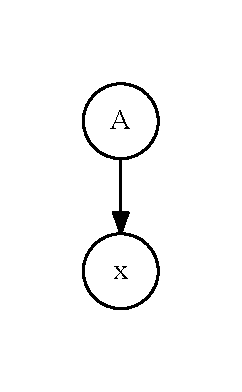
\includegraphics[width=0.2\textwidth]{pictures/tree1.pdf}
 \caption{The derivation tree of the height $h = 1$ for the string $x = l(\pi)$.}
 \label{tree1}
\end{figure}

\textbf{Inductive step}: Assume that the statement of the lemma holds for any $k \leq (p - 1)$ and show that it also holds for $k = p$ where $p \geq 2$. For any $i, j$ and for any non-terminal $A \in N$, $$A \in a^{(p)}_{i,j} \text{ iff } A \in a^{(p-1)}_{i,j} \text{ or } A \in (a^{(p-1)} \times a^{(p-1)})_{i,j},$$ since $$a^{(p)} = a^{(p-1)} \cup (a^{(p-1)} \times a^{(p-1)}).$$

Let $A \in a^{(p-1)}_{i,j}$. By the inductive hypothesis, $A \in a^{(p-1)}_{i,j}$ iff $(i,j) \in R_A$ and there exists $i \pi j$, such that there is a derivation tree of the height $h \leq (p-1)$ for the string $l(\pi)$ and a context-free grammar $G_A = (N,\Sigma,P,A)$. The statement of the lemma holds for $k = p$ since the height $h$ of this tree is also less than or equal to $p$.

Let $A \in (a^{(p-1)} \times a^{(p-1)})_{i,j}$. By the definition of the binary operation $(\cdot)$ on arbitrary subsets, $A \in (a^{(p-1)} \times a^{(p-1)})_{i,j}$ iff there are $r$, $B \in a^{(p-1)}_{i,r}$ and $C \in a^{(p-1)}_{r,j}$, such that $(A \rightarrow B C) \in P$. Hence, by the inductive hypothesis, there are $i \pi_1 r$ and $r \pi_2 j$, such that $(i,r) \in R_B$ and $(r,j) \in R_C$, and there are the derivation trees $T_B$ and $T_C$ of heights $h_1 \leq (p-1)$ and $h_2 \leq (p-1)$ for the strings $w_1 = l(\pi_1)$, $w_2 = l(\pi_2)$ and the context-free grammars $G_B$, $G_C$ respectively. Thus, the concatenation of paths $\pi_1$ and $\pi_2$ is $i \pi j$, where $(i,j) \in R_A$ and there is a derivation tree of the height $h = 1 + max(h_1, h_2)$, shown in Figure~\ref{tree2}, for the string $w = l(\pi)$ and a context-free grammar $G_A$.

\begin{figure}[h!]
 \centering
 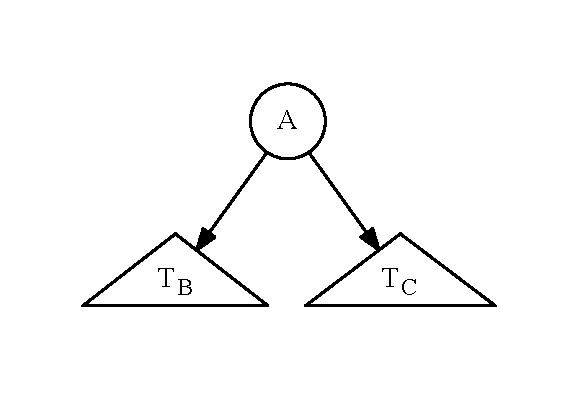
\includegraphics[width=0.8\textwidth]{pictures/tree2.pdf}
 \caption{The derivation tree of the height $h = 1 + max(h_1, h_2)$ for the string $w = l(\pi)$, where $T_B$ and $T_C$ are the derivation trees for strings $w_1$ and $w_2$ respectively.}
 \label{tree2}
\end{figure}

The statement of the lemma holds for $k = p$ since the height $h = 1 + max(h_1, h_2) \leq p$. This completes the proof of the lemma.
\end{proof}

\begin{mytheorem}\label{thm:correct}
 Let $D = (V,E)$ be a graph and let $G =(N,\Sigma,P)$ be a grammar. Then for any $i, j$ and for any non-terminal $A \in N$, $A \in a^{cf}_{i,j}$ iff $(i,j) \in R_A$.
\end{mytheorem}
\begin{proof}

Since the matrix $a^{cf} = a^{(1)} \cup a^{(2)} \cup \cdots,$ for any $i, j$ and for any non-terminal $A \in N$, $A \in a^{cf}_{i,j}$ iff there is $k \geq 1$, such that $A \in a^{(k)}_{i,j}$. By the lemma~\ref{lemma:cf}, $A \in a^{(k)}_{i,j}$ iff $(i,j) \in R_A$ and there is $i \pi j$, such that there is a derivation tree of the height $h \leq k$ for the string $l(\pi)$ and a context-free grammar $G_A = (N,\Sigma,P,A)$. This completes the proof of the theorem.
\end{proof}

We can, therefore, determine whether $(i,j) \in R_A$ by asking whether $A \in a^{cf}_{i,j}$. Thus, we show how the context-free relations $R_A$ can be calculated by computing the transitive closure $a^{cf}$ of the matrix $a$.



\subsection{The algorithm} \label{section_algorithm}
In this section, we introduce an algorithm for calculating the transitive closure $a^{cf}$ which was discussed in Section~\ref{section_reducing}.

Let $D = (V, E)$ be the input graph and $G = (N,\Sigma,P)$ be the input grammar.

\begin{algorithm}[H]
\begin{algorithmic}[1]
\caption{Context-free recognizer for graphs}
\label{alg:graphParse}
\Function{contextFreePathQuerying}{D, G}
    
    \State{$n \gets$ the number of nodes in $D$}
    \State{$E \gets$ the directed edge-relation from $D$}
    \State{$P \gets$ the set of production rules in $G$}
    \State{$T \gets$ the matrix $n \times n$ in which each element is $\varnothing$}
    \ForAll{$(i,x,j) \in E$}
    \Comment{Matrix initialization}
        \State{$T_{i,j} \gets T_{i,j} \cup \{A~|~(A \rightarrow x) \in P \}$}
    \EndFor    
    \While{matrix $T$ is changing}
       
        \State{$T \gets T \cup (T \times T)$}
        \Comment{Transitive closure $T^{cf}$ calculation} 
    \EndWhile
\State \Return $T$
\EndFunction
\end{algorithmic}
\end{algorithm}

Note that the matrix initialization in lines \textbf{6-7} of the Algorithm~\ref{alg:graphParse} can handle arbitrary graph $D$. For example, if a graph $D$ contains multiple edges $(i,x_1,j)$ and $(i,x_2,j)$ then both the elements of the set $\{A~|~(A \rightarrow x_1) \in P \}$ and the elements of the set $\{A~|~(A \rightarrow x_2) \in P \}$ will be added to $T_{i,j}$.

We need to show that the Algorithm~\ref{alg:graphParse} terminates in a finite number of steps. Since each element of the matrix $T$ contains no more than $|N|$ non-terminals, the total number of non-terminals in the matrix $T$ does not exceed $|V|^2|N|$. Therefore, the following theorem holds.

\begin{mytheorem}\label{thm:finite}
 Let $D = (V,E)$ be a graph and let $G =(N,\Sigma,P)$ be a grammar. The Algorithm~\ref{alg:graphParse} terminates in a finite number of steps. 
\end{mytheorem}
\begin{proof}
It is sufficient to show, that the operation in the line \textbf{9} of the Algorithm~\ref{alg:graphParse} changes the matrix $T$ only finite number of times. Since this operation can only add non-terminals to some elements of the matrix $T$, but not remove them, it can change the matrix $T$ no more than $|V|^2|N|$ times.
\end{proof}

Denote the number of elementary operations executed by the algorithm of multiplying two $n \times n$ Boolean matrices as $BMM(n)$. According to Valiant, the matrix multiplication operation in the line \textbf{9} of the Algorithm~\ref{alg:graphParse} can be calculated in $O(|N|^2 BMM(|V|))$. Denote the number of elementary operations executed by the matrix union operation of two $n \times n$ Boolean matrices as $BMU(n)$. Similarly, it can be shown that the matrix union operation in the line \textbf{9} of the Algorithm~\ref{alg:graphParse} can be calculated in $O(|N|^2 BMU(n))$. Since the line \textbf{9} of the Algorithm~\ref{alg:graphParse} is executed no more than $|V|^2|N|$ times, the following theorem holds.

\begin{mytheorem}\label{thm:time}
 Let $D = (V,E)$ be a graph and let $G =(N,\Sigma,P)$ be a grammar. The Algorithm~\ref{alg:graphParse} calculates the transitive closure $T^{cf}$ in $O(|V|^2|N|^3(BMM(|V|) + BMU(|V|)))$.
\end{mytheorem}

We also provide the worst-case example, for which the time complexity in terms of the graph size provided by Theorem~\ref{thm:time} cannot be improved. This example is based on the context-free grammar $G = (N, \Sigma, P)$ where:
\begin{itemize}
	\item the set of non-terminals $N = \{S\}$;
	\item the set of terminals $\Sigma = \{a, b\}$;
	\item the set of production rules $P$ is presented on Figure~\ref{ProductionRulesWorsCaseExample}.
\end{itemize}

\begin{figure}[h]
	\[
	\begin{array}{rccl}
	0: & S & \rightarrow & \text{\emph{a}} \ S \ \text{\emph{b}} \\
	1: & S & \rightarrow & \text{\emph{a}} \ \text{\emph{b}} \\ 
	\end{array}
	\]
	\caption{Production rules for the worst-case example.}
	\label{ProductionRulesWorsCaseExample}
\end{figure}

Let the size $|N|$ of the grammar $G$ be a constant. The worst-case time complexity is reached by running this query on the double-cyclic graph where:
\begin{itemize}
	\item one of the cycles having $u = 2^k + 1$ edges labeled with $a$;
	\item another cycle having $v = 2^k$ edges labeled with $b$;
	\item the two cycles are connected via a shared node $m$.
\end{itemize}

A small example of such graph with $k = 1$, $u = 3$, $v = 2$, and $m = 0$ is presented on Figure~\ref{worst_case_graph}.

\begin{figure}[h]
	\[
	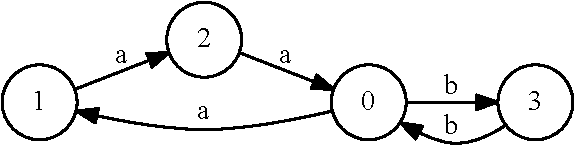
\includegraphics[width=0.8\textwidth]{pictures/worst_case_graph.pdf}
	\]
	\caption{An example of the graph for the worst-case time complexity.}
	\label{worst_case_graph}
\end{figure}

The shortest path $\pi$ from the node $m$ to the node $m$, whose labeling forms a string from the language $L(G_S)=\{a^n b^n; n \geq 1\}$, has a length $l = 2*u*v$, since $u = 2^k + 1$ and $v = 2^k$ are coprime, and string $s$, formed by this path, consists of $u*v$ labels $a$ and $u*v$ labels $b$. The string $s = l(\pi)$ has a derivation tree according to a context-free grammar $G_S$ of the minimal height $h = 2*u*v$ among all the paths from the node $m$ to the node $m$ in this double-cyclic graph. Therefore, if we run the worst-case example query on this graph, then the operation in the line \textbf{9} of the Algorithm~\ref{alg:graphParse} changes the matrix $T$ at least $h = 2*u*v$ times. Hence, the Algorithm~\ref{alg:graphParse} computes this query in $O(|V|^2(BMM(|V|) + BMU(|V|)))$, since $|V| = (u + v - 1) = 2*v$ and $h = 2*u*v > 2*v*v = |V|^2 / 4 = O(|V|^2)$.


\subsection{An example} \label{section_example}
In this section, we provide a step-by-step demonstration of the proposed algorithm. For this, we consider the classical \textit{same-generation query}~\cite{FndDB}.

The \textbf{example query} is based on the context-free grammar $G = (N, \Sigma, P)$ where:
\begin{itemize}
    \item The set of non-terminals $N = \{S\}$.
    \item The set of terminals $$\Sigma = \{subClassOf, subClassOf^{-1}, type, type^{-1}\}.$$
    \item The set of production rules $P$ is presented in Figure~\ref{ProductionRulesExampleQuery}.
\end{itemize}

\begin{figure}[h]
   \[
\begin{array}{rccl}
   0: & S & \rightarrow & \text{\textit{subClassOf}}^{-1} \ S \ \text{\textit{subClassOf}} \\ 
   1: & S & \rightarrow & \text{\textit{type}}^{-1} \ S \ \text{\textit{type}} \\ 
   2: & S & \rightarrow & \text{\textit{subClassOf}}^{-1} \ \text{\textit{subClassOf}} \\ 
   3: & S & \rightarrow & \text{\textit{type}}^{-1} \ \text{\textit{type}} \\ 
\end{array}
\]
\caption{Production rules for the example query grammar.}
\label{ProductionRulesExampleQuery}
\end{figure}

Since the proposed algorithm processes only grammars in Chomsky normal form, we first transform the grammar $G$ into an equivalent grammar $G' = (N', \Sigma', P')$ in normal form, where:
\begin{itemize}
    \item The set of non-terminals $N' = \{S, S_1, S_2, S_3, S_4, S_5, S_6\}$.
    \item The set of terminals $$\Sigma' = \{subClassOf, subClassOf^{-1}, type, type^{-1}\}.$$
    \item The set of production rules $P'$ is presented in Figure~\ref{ProductionRulesExampleQueryCNF}.
\end{itemize}

\begin{figure}[h]
   \[
\begin{array}{rccl}
   0: & S & \rightarrow & S_1 \ S_5 \\
   1: & S & \rightarrow & S_3 \ S_6 \\
   2: & S & \rightarrow & S_1 \ S_2 \\
   3: & S & \rightarrow & S_3 \ S_4 \\
   4: & S_5 & \rightarrow & S \ S_2 \\
   5: & S_6 & \rightarrow & S \ S_4 \\
   6: & S_1 & \rightarrow & \text{\textit{subClassOf}}^{-1} \\ 
   7: & S_2 & \rightarrow & \text{\textit{subClassOf}} \\ 
   8: & S_3 & \rightarrow & \text{\textit{type}}^{-1} \\
   9: & S_4 & \rightarrow & \text{\textit{type}} \\ 
\end{array}
\]
\caption{Production rules for the example query grammar in normal form.}
\label{ProductionRulesExampleQueryCNF}
\end{figure}

We run the query on a graph presented in Figure~\ref{ExampleQueryGraph}.

\begin{figure}[h]
\[
    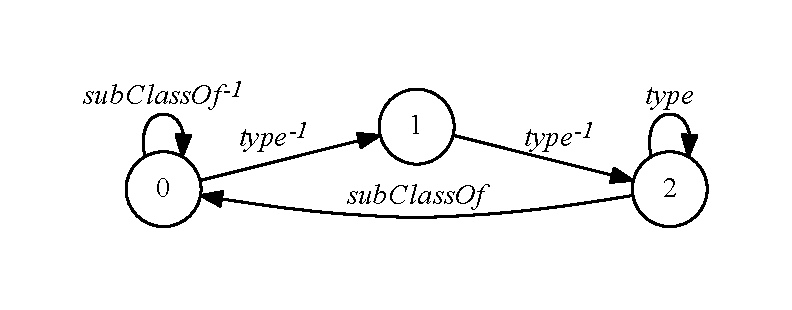
\includegraphics[width=0.8\textwidth]{pictures/ExampleGraph.pdf}
\]
\caption{An input graph for the example query.}
\label{ExampleQueryGraph}
\end{figure}

We provide a step-by-step demonstration of the work with the given graph $D$ and grammar $G'$ of the Algorithm~\ref{alg:graphParse}. After the matrix initialization in lines \textbf{6-7} of the Algorithm~\ref{alg:graphParse}, we have a matrix $T_0$ presented in Figure~\ref{ExampleQueryInitMatrix}.

\begin{figure}[h]
\[
T_0 = \begin{pmatrix}
    \{S_1\} & \{S_3\} & \varnothing \\ \varnothing & \varnothing & \{S_3\} \\ \{S_2\} & \varnothing & \{S_4\}
\end{pmatrix}
\]
\caption{The initial matrix for the example query.}
\label{ExampleQueryInitMatrix}
\end{figure}

Let $T_i$ be the matrix $T$ obtained after executing the loop in lines \textbf{8-9} of the Algorithm~\ref{alg:graphParse} $i$ times. The calculation of the matrix $T_1$ is shown in Figure~\ref{ExampleQueryFirstIteration}.

\begin{figure}[h]
\[
T_0 \times T_0 = \begin{pmatrix}
    \varnothing & \varnothing & \varnothing \\ \varnothing & \varnothing & \{S\} \\ \varnothing & \varnothing & \varnothing
\end{pmatrix}
\]

\[
T_1 = T_0 \cup (T_0 \times T_0) = \begin{pmatrix}
    \{S_1\} & \{S_3\} & \varnothing \\ \varnothing & \varnothing & \{S_3, S\} \\ \{S_2\} & \varnothing & \{S_4\}
\end{pmatrix}
\]
\caption{The first iteration of computing the transitive closure for the example query.}
\label{ExampleQueryFirstIteration}
\end{figure}

When the algorithm at some iteration finds new paths in the graph $D$, then it adds corresponding nonterminals to the matrix $T$. For example, after the first loop iteration, non-terminal $S$ is added to the matrix $T$. This non-terminal is added to the element with a row index $i = 1$ and a column index $j = 2$. This means that there is $i\pi j$ (a path $\pi$ from the node 1 to the node 2), such that $S \xrightarrow{*} l(\pi)$. For example, such a path consists of two edges with labels $type^{-1}$ and $type$, and thus $S \xrightarrow{*} type^{-1} \ type$.

The calculation of the transitive closure is completed after $k$ iterations when a fixpoint is reached: $T_{k-1} = T_k$. For the example query, $k = 6$ since $T_6 = T_5$. The remaining iterations of computing the transitive closure are presented in Figure~\ref{ExampleQueryFinalIterations}.

\begin{figure}[h]
\[
T_2 = \begin{pmatrix}
    \{S_1\} & \{S_3\} & \varnothing \\ \{S_5\} & \varnothing & \{S_3, S, S_6\} \\ \{S_2\} & \varnothing & \{S_4\}
\end{pmatrix}
\]

\[
T_3 = \begin{pmatrix}
    \{S_1\} & \{S_3\} & \{S\} \\ \{S_5\} & \varnothing & \{S_3, S, S_6\} \\ \{S_2\} & \varnothing & \{S_4\}
\end{pmatrix}
\]

\[
T_4 = \begin{pmatrix}
    \{S_1, S_5\} & \{S_3\} & \{S, S_6\} \\ \{S_5\} & \varnothing & \{S_3, S, S_6\} \\ \{S_2\} & \varnothing & \{S_4\}
\end{pmatrix}
\]

\[
T_5 = \begin{pmatrix}
    \{S_1, S_5, S\} & \{S_3\} & \{S, S_6\} \\ \{S_5\} & \varnothing & \{S_3, S, S_6\} \\ \{S_2\} & \varnothing & \{S_4\}
\end{pmatrix}
\]
\caption{Remaining states of the matrix $T$.}
\label{ExampleQueryFinalIterations}
\end{figure}

Thus, the result of the Algorithm~\ref{alg:graphParse} for the example query is the matrix $T_5 = T_6$. Now, after constructing the transitive closure, we can construct the context-free relations $R_A$. These relations for each non-terminal of the grammar $G'$ are presented in Figure~\ref{ExampleQueryCFRelations}.

\begin{figure}[h]
\begin{eqnarray*}
R_S&=&\{(0,0),(0,2),(1,2)\},\\
R_{S_1}&=&\{(0,0)\},\\
R_{S_2}&=&\{(2,0)\}, \\
R_{S_3}&=&\{(0,1), (1,2)\}, \\
R_{S_4}&=&\{(2,2)\}, \\
R_{S_5}&=&\{(0,0), (1,0)\}, \\
R_{S_6}&=&\{(0,2), (1,2)\}.
\end{eqnarray*}
\caption{Context-free relations for the example query.}
\label{ExampleQueryCFRelations}
\end{figure}

By the context-free relation $R_S$, we can conclude that there are paths in a graph $D$ only from the node 0 to the node 0, from the node 0 to the node 2 or from the node 1 to the node 2, corresponding to the context-free grammar $G_S$. This conclusion is based on the fact that a grammar $G'_S$ is equivalent to the grammar $G_S$ and $L(G_S) = L(G_S')$.

\section{Экспериментальное исследование}
Предложенный механизм диагностики ошибок был реализован на платформе .NET как часть проекта YaccConstructor; основным языком разработки являлся F\#~\cite{FSharp}. Данная реализация является модификацией ранее реализованного в рамках проекта алгоритма ослабленного синтаксического анализа регулярной аппроксимации динамически формируемого выражения.

Модифицированный алгоритм был протестирован на серии тестов с целью проверки работоспособности. Данные тесты проверяли, что алгоритм строит корректные множества $errors$ и $probErrors$ ребер входного графа. Для каждого теста специфицировалась грамматика на языке YARD и в явном виде задавался граф конечного автомата, ребра которого были промаркированы лексемами входной грамматики. Входные графы для данных тестов содержали как ветвления, так и циклы. На всех тестах модифицированный алгоритм корректно строил множества $errors$ и $probErrors$. Кроме того, на всех тестах, входные графы которых не содержали циклов, модифицированный алгоритм точно определял все ошибочные ребра входного графа, то есть $probErrors$, в данном случае, являлось пустым множеством.

Также на нескольких сериях синтетических тестов была протестирована производительность модифицированного алгоритма. Анализ промышленного проекта по миграции базы данных с MS-SQL Server 2005 на Oracle 11gR2 показал, что запросы часто формируются конкатенацией фрагментов, каждый из которых формируется с помощью ветвлений или циклов. Ниже приведена входная грамматика, использованная в данных тестах:
$$
\begin{array}{crcl}
& start\_rule &::=& s \\
& s & ::= & s \mbox{\texttt{ PLUS }} \mbox{\texttt{n}}\\
& n & ::= & \mbox{\texttt{ONE | }} \mbox{\texttt{TWO | }} \mbox{\texttt{THREE | }} \mbox{\texttt{FIVE | }} \mbox{\texttt{SIX | }} \mbox{\texttt{SEVEN}}
\end{array}
$$
Входные графы представляли собой конкатенацию базовых блоков без циклов. Каждая серия тестов характеризовалась тремя параметрами: 
\begin{itemize}
  \item $height$~--- количество ветвлений в базовом блоке;
  \item $length$~--- максимальное количество повторений базовых блоков;
  \item $errorBranches$~--- количество веток в базовом блоке, содержащих ошибочное ребро (на рис.~\ref{block} изображен базовый блок без ошибочных ребер, а на рис.~\ref{errorBlock} --- базовый блок с двумя выделенными ошибочными ребрами).
\end{itemize}

\begin{figure}[h!]
 \centering
 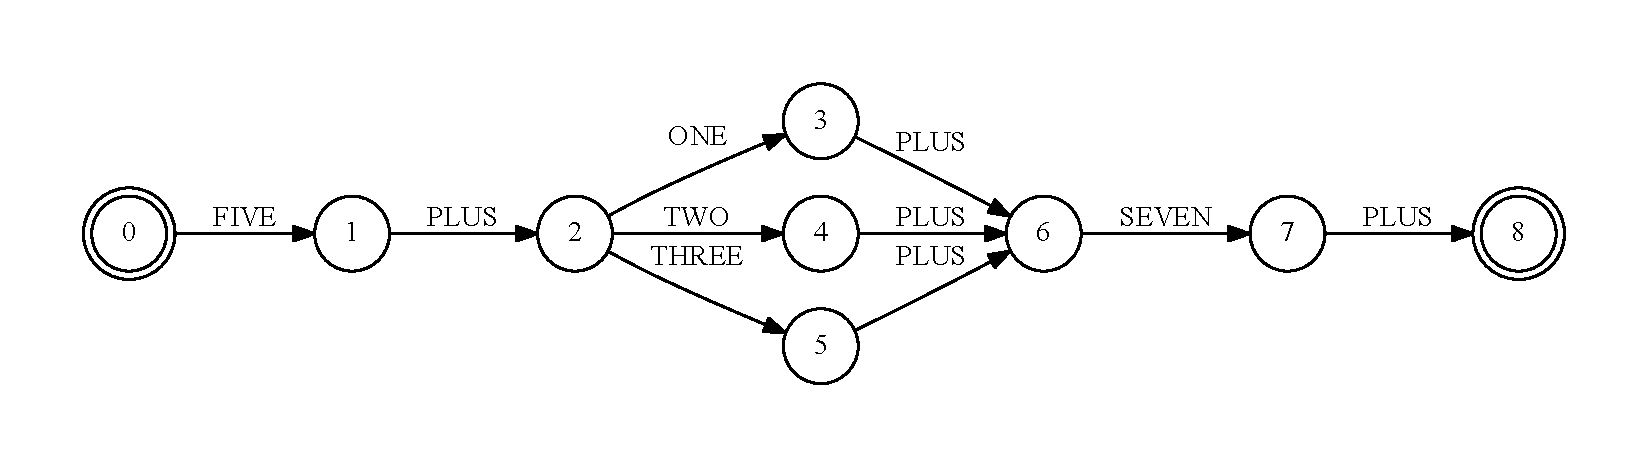
\includegraphics[width=\textwidth]{Azimov/pictures/block_black.pdf}
 \caption{Базовый блок при $height=3, errorBranches=0$}
 \label{block}
\end{figure}

\begin{figure}[h!]
 \centering
 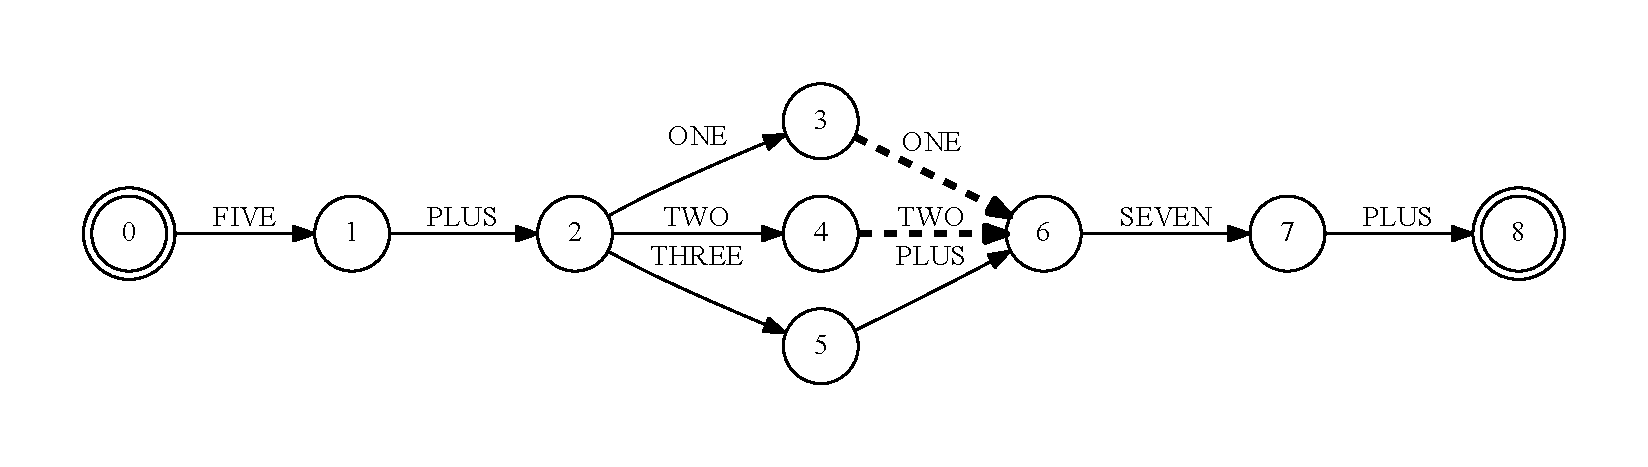
\includegraphics[width=\textwidth]{Azimov/pictures/errorBlock_black.pdf}
 \caption{Базовый блок при $height=3, errorBranches=2$}
 \label{errorBlock}
\end{figure}

Замеры времени работы алгоритмов проводились на машине со следующими техническими характеристиками: Intel(R) Core(TM) i7-3630QM CPU @ 2.40GHz, RAM: 8.0~GB, процессор x64.

\begin{figure}[H]
 \centering
 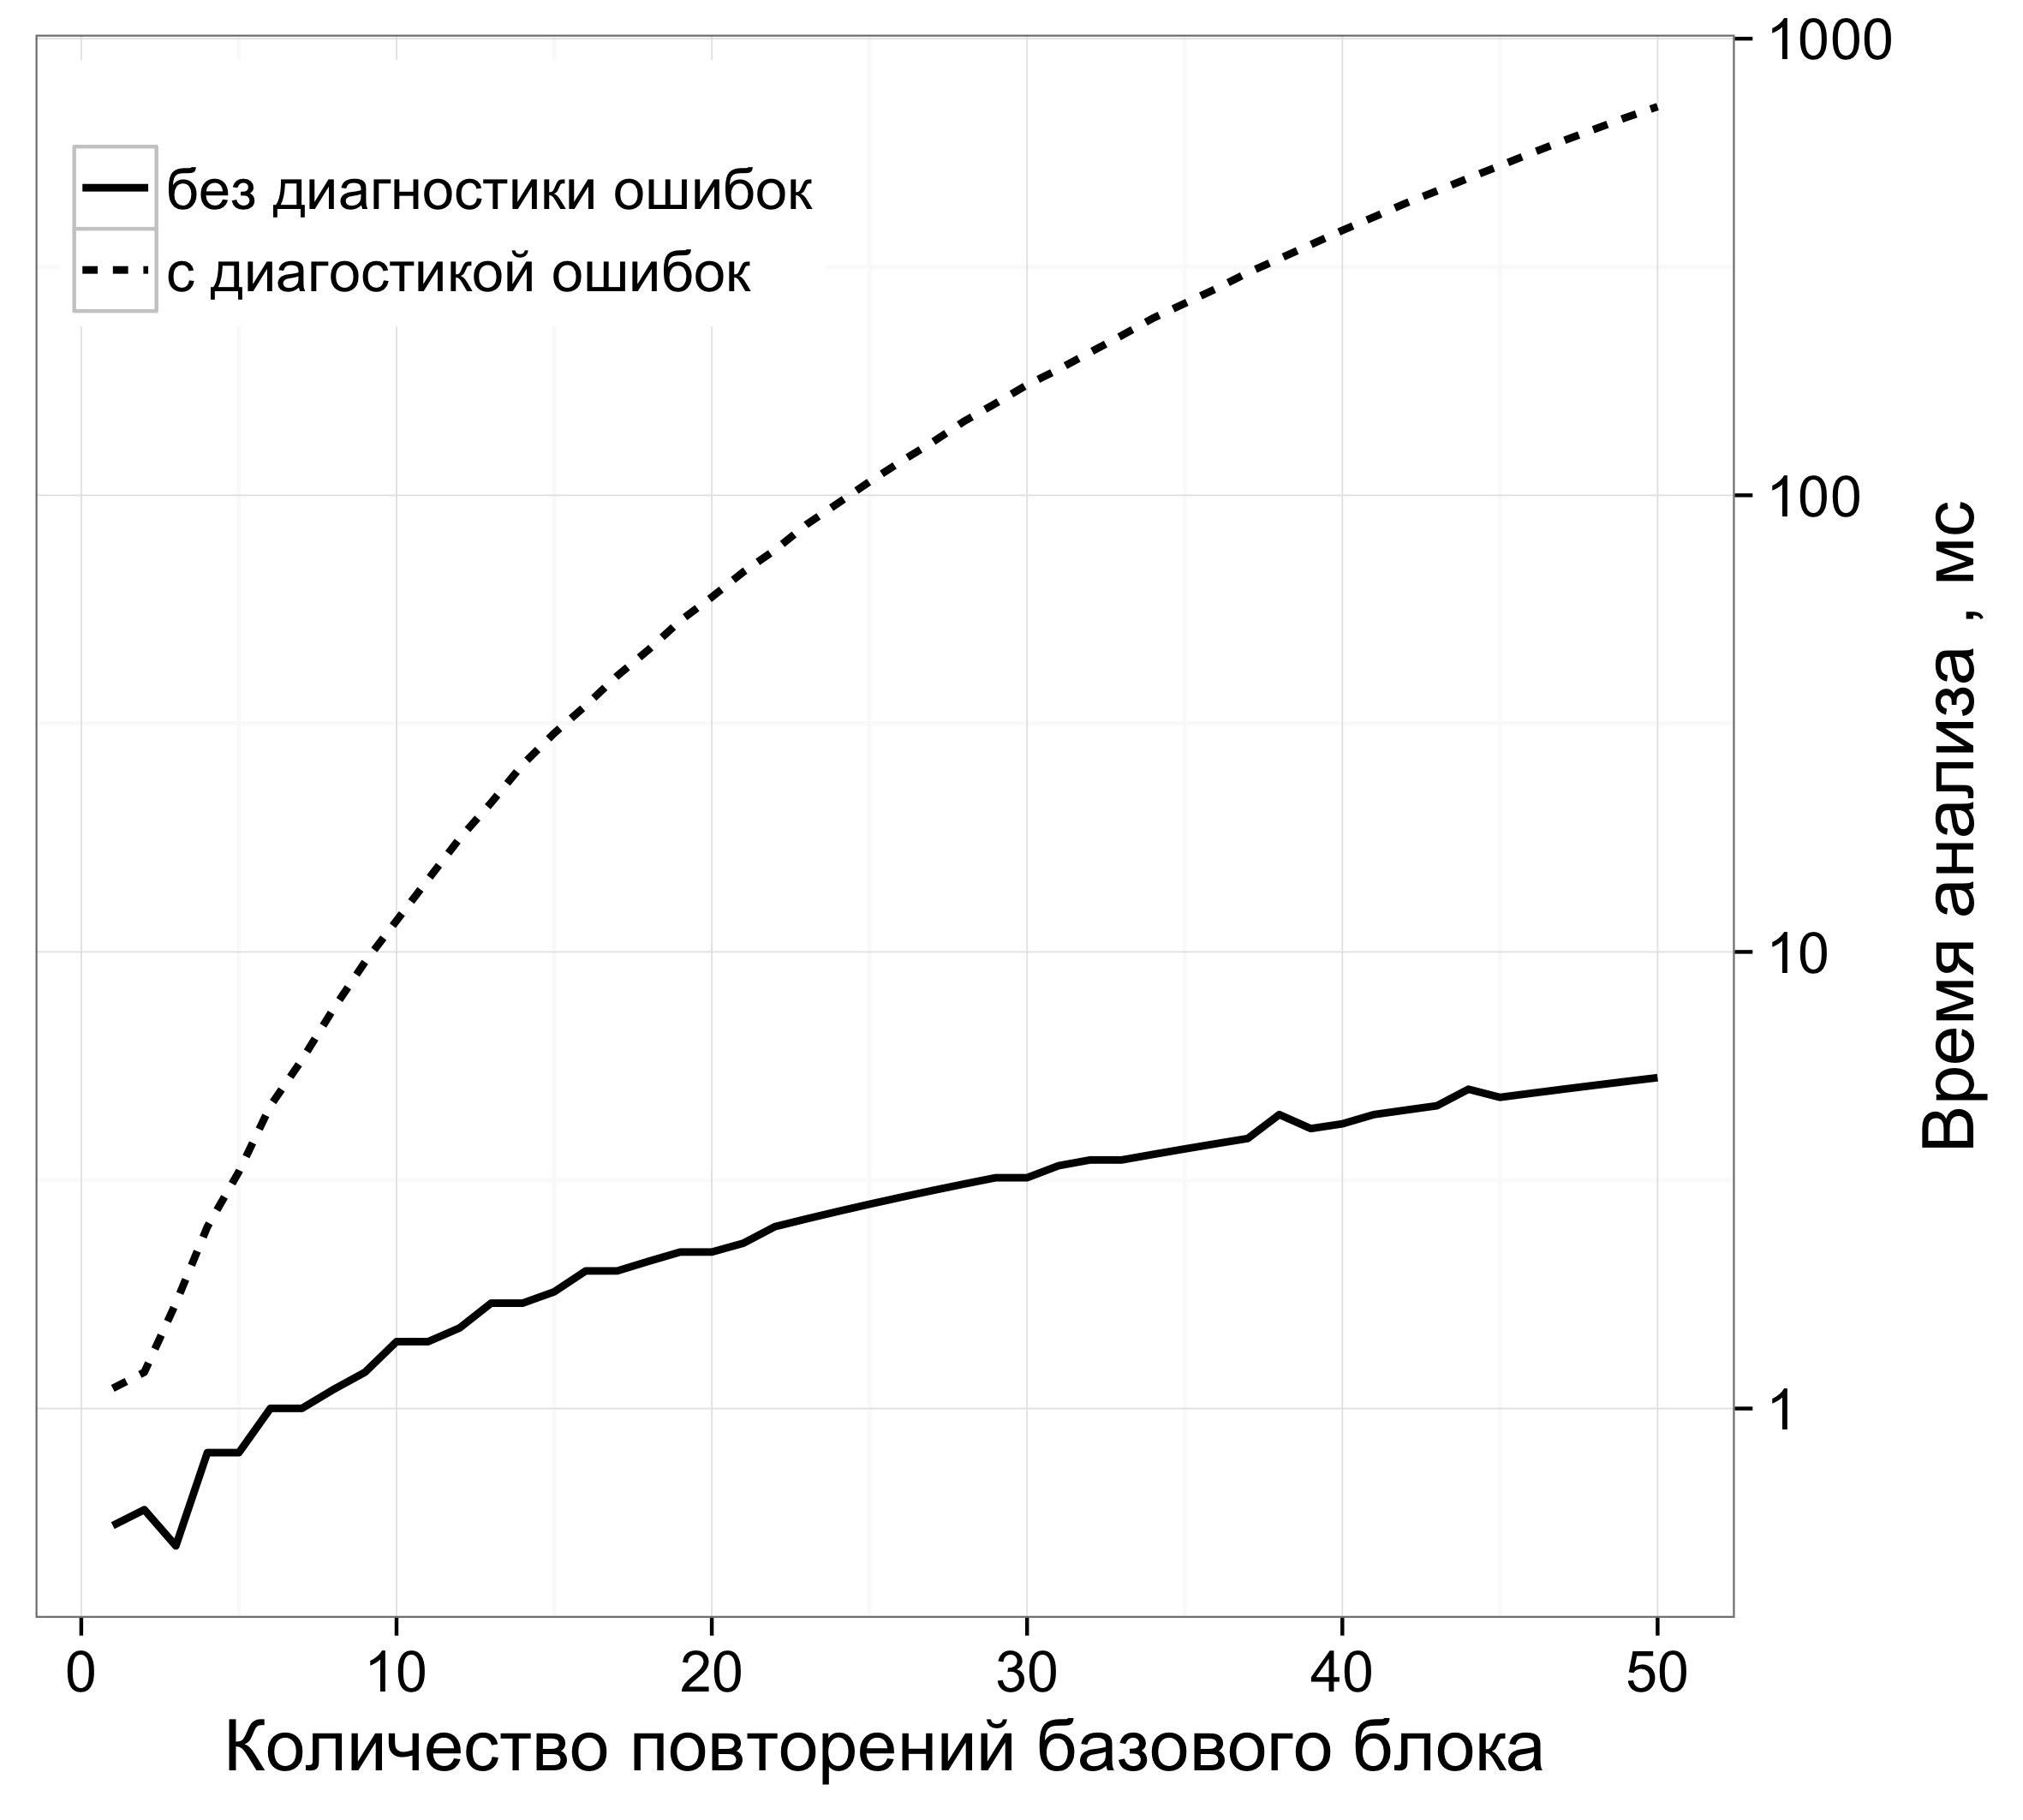
\includegraphics[width=0.9\textwidth]{Azimov/pictures/compare_black.png}
 \caption{Сравнение времени работы алгоритма синтаксического анализа до и после модификаций, при $height=4, errors=0$}
 \label{compare}
\end{figure}


Каждая серия объединяет набор из 50 тестов, каждый из которых содержит одинаковое количество ветвлений в базовом блоке, при этом количество повторений блока совпадает с порядковым номером теста ($length = i$, для теста с номером $i$). Для каждого теста измерялось время, затраченное на синтаксический анализ. Измерения проводились 10 раз, после чего усреднялись. График, представленный на рис.~\ref{compare}, иллюстрирует сравнение времени работы алгоритма синтаксического анализа до и после модификаций. Можно заметить, что выполненная модификация существенно увеличивает продолжительность анализа. Причина этого в том, что выполненная модификация является прототипом, а в будущем планируется улучшить производительность путем улучшения реализации. График на рис.~\ref{withErrors} демонстрирует зависимость времени работы модифицированного алгоритма от количества повторений базового блока и количества веток, содержащих ошибочное ребро, в каждом из них. Наблюдается уменьшение времени работы модифицированного алгоритма при увеличении количества ошибочных ребер. Одной из причин этого является уменьшение количества корректных префиксов внутреннего графа при увеличении количества ошибочных ребер.

\begin{figure}[H]
 \centering
 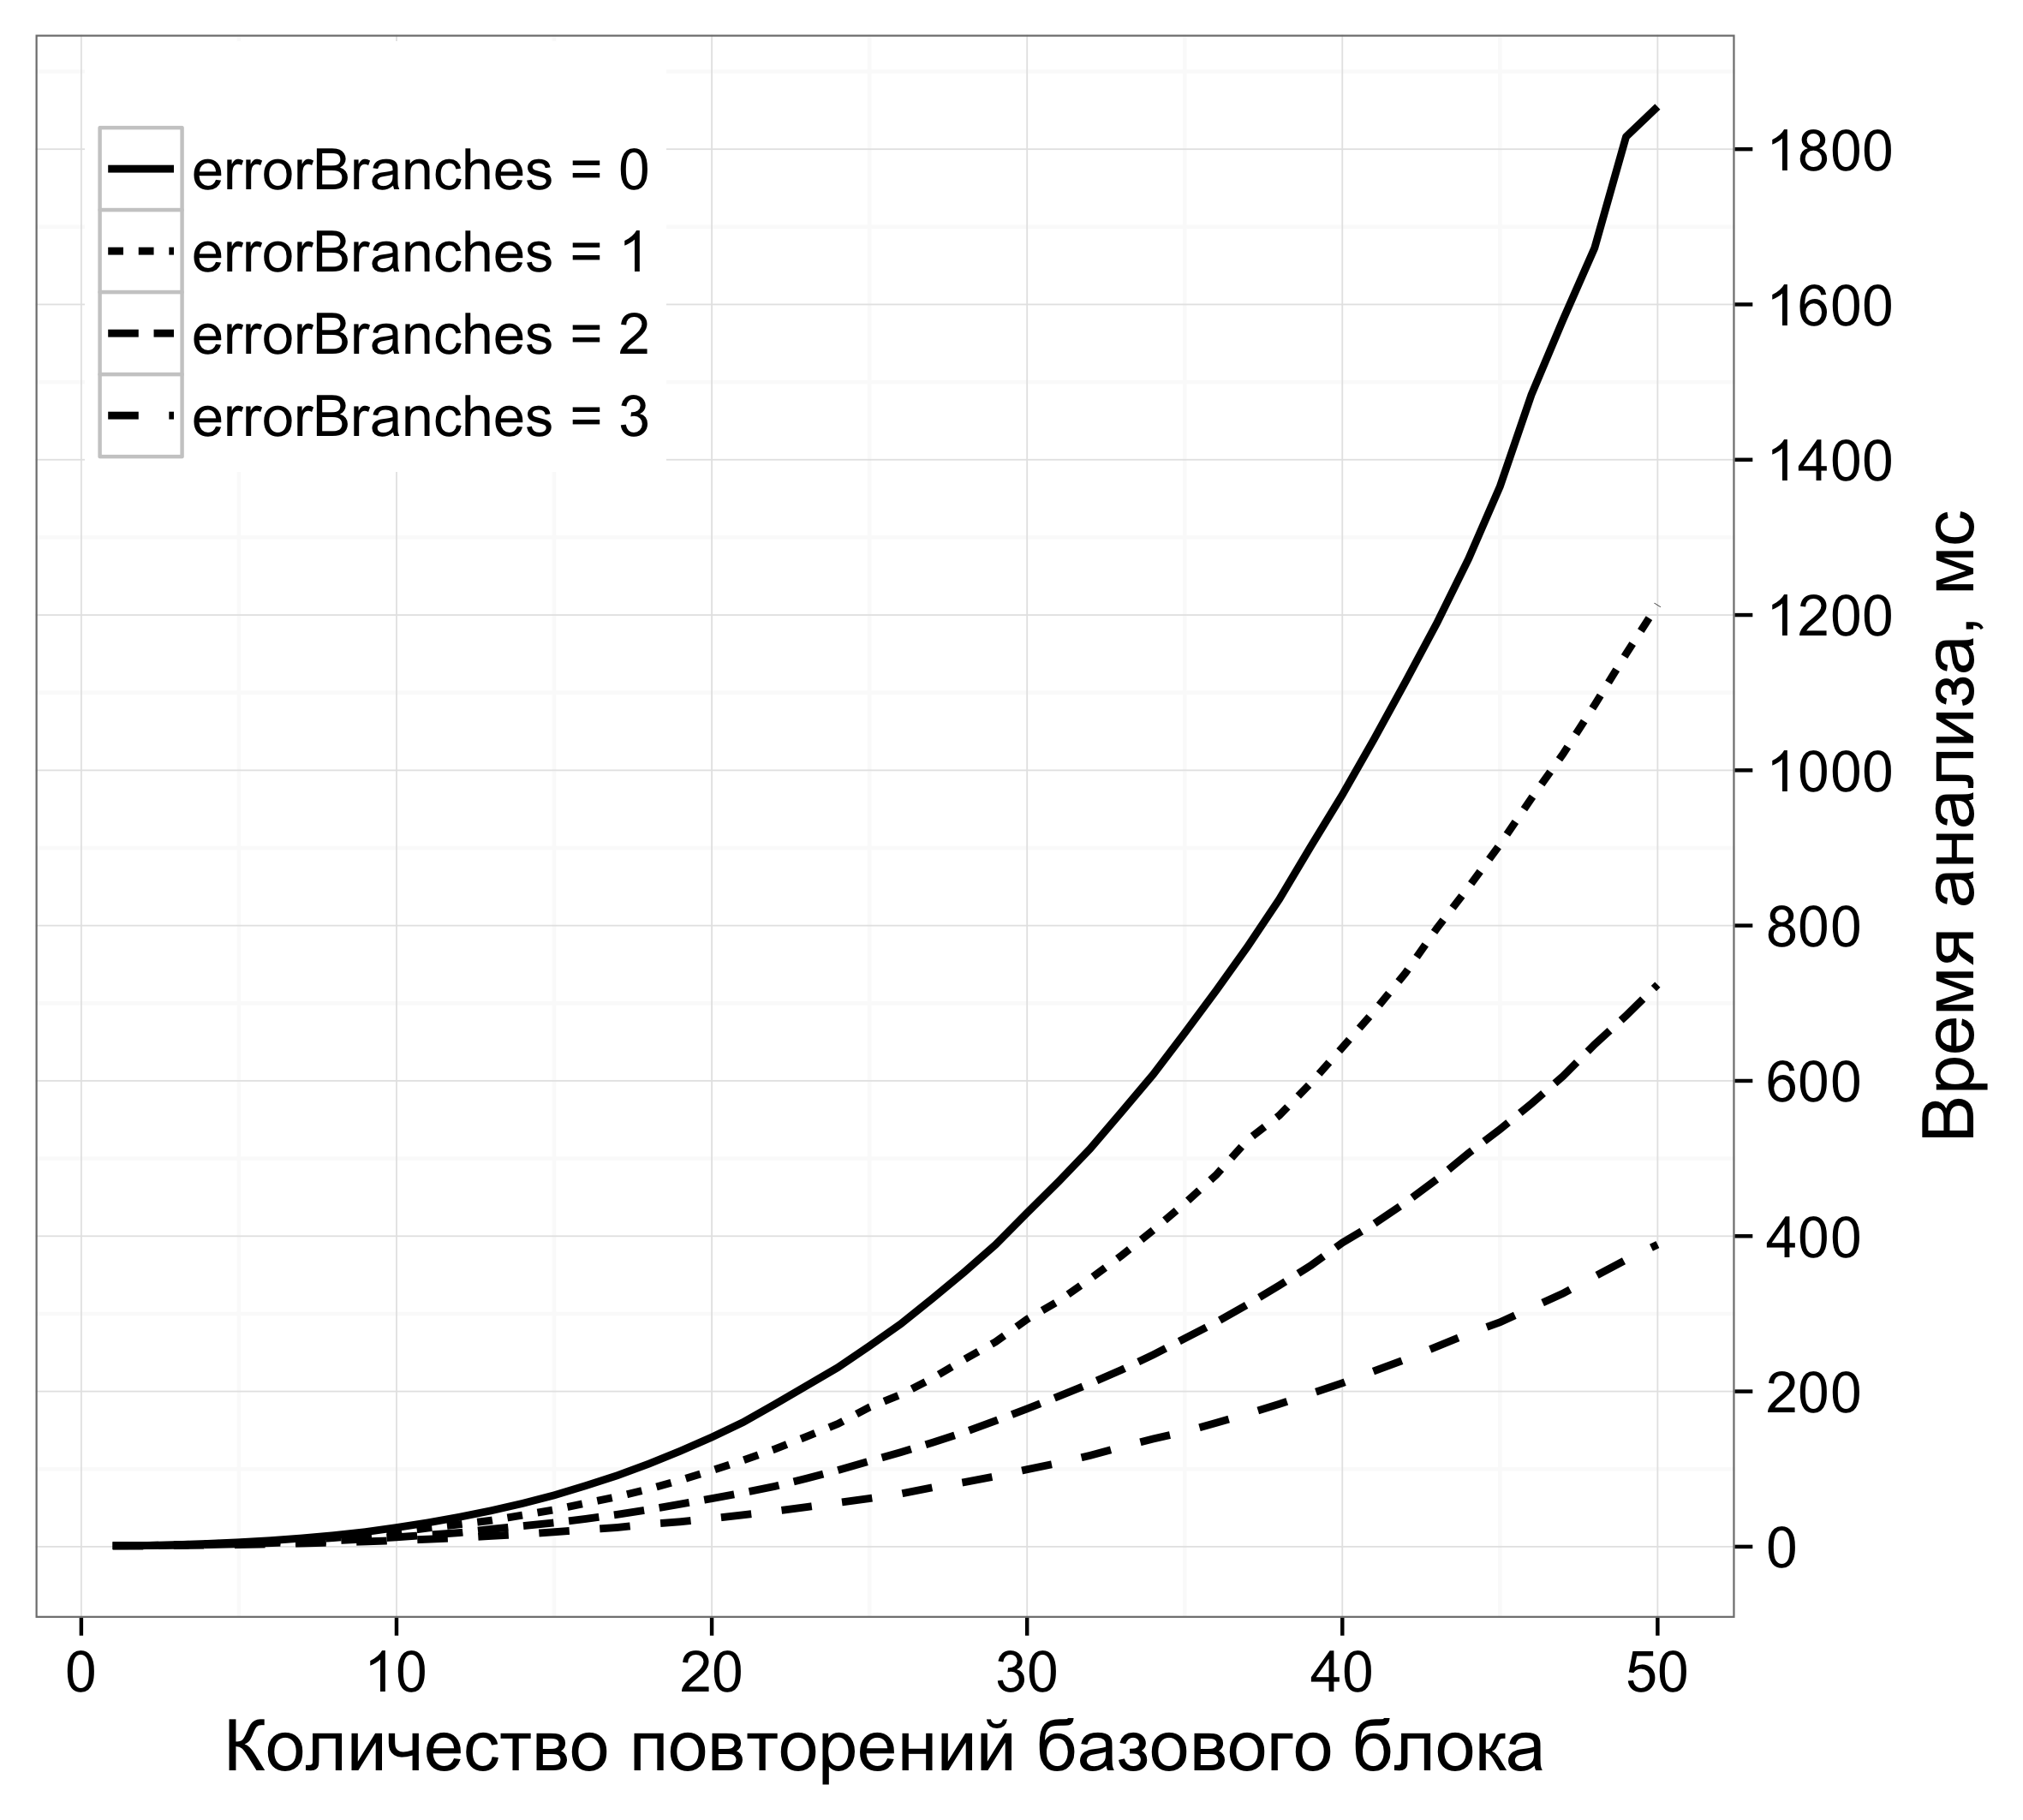
\includegraphics[width=0.9\textwidth]{Azimov/pictures/error_branches4_black.png}
 \caption{Зависимость времени работы модифицированного алгоритма от размера входного графа и количества ошибочных ребер при $height=6$}
 \label{withErrors}
\end{figure}

\section{Заключение}

В данной работе описан подход к композициональному символьному исполнению без раскрутки. Была предложена концепция композициональной памяти с символьной адресацией. Был доказан некоторый набор свойств КСП, дающий основание для подхода в стиле систем переписывания, где символьные кучи могут сами выступать как символы. Это даёт возможность автоматически порождать уравнения на состояния, решения которых в точности отражают поведения функций, работающих с динамической памятью. Было показано как свести задачу решения уравнений на состояния к задаче проверки безопасности чистых функций второго порядка.

Данная работа нацелена на теоретические основания композиционального анализа динамической памяти. Мы оставляем апробацию этого подхода на будущее. Другим направлением будущих исследований может быть расширение нашего формализма на композициональный анализ параллельных программ.

%\setmonofont[Mapping=tex-text]{CMU Typewriter Text}
%\bibliographystyle{ugost2008ls}
%\bibliography{diploma.bib}

\begin{thebibliography}{10}
\def\selectlanguageifdefined#1{
\expandafter\ifx\csname date#1\endcsname\relax
\else\selectlanguage{#1}\fi}
\providecommand*{\href}[2]{{\small #2}}
\providecommand*{\url}[1]{{\small #1}}
\providecommand*{\BibUrl}[1]{\url{#1}}
\providecommand{\BibAnnote}[1]{}
\providecommand*{\BibEmph}[1]{#1}
\ProvideTextCommandDefault{\cyrdash}{\iflanguage{russian}{\hbox
  to.8em{--\hss--}}{\textemdash}}
\providecommand*{\BibDash}{\ifdim\lastskip>0pt\unskip\nobreak\hskip.2em plus
  0.1em\fi
\cyrdash\hskip.2em plus 0.1em\ignorespaces}
\renewcommand{\newblock}{\ignorespaces}

\bibitem{Afroozeh2015gss}
\selectlanguageifdefined{english}
\BibEmph{Afroozeh~Ali, Izmaylova~Anastasia}.
  \href{http://dx.doi.org/10.1007/978-3-662-46663-6\_5}{Faster, Practical GLL
  Parsing}~// Compiler Construction: 24th International Conference, CC 2015,
  Held as Part of the European Joint Conferences on Theory and Practice of
  Software, ETAPS 2015, London, UK, April 11-18, 2015, Proceedings~/ Ed.\ by\
  Bj{\"o}rn~Franke. \BibDash
\newblock Berlin, Heidelberg~: Springer Berlin Heidelberg, 2015. \BibDash
\newblock P.~89--108. \BibDash
\newblock
  ISBN:~\href{http://isbndb.com/search-all.html?kw=978-3-662-46663-6}{978-3-662-46663-6}.
  \BibDash
\newblock URL: \BibUrl{http://dx.doi.org/10.1007/978-3-662-46663-6\_5}.

\bibitem{Arimura}
\selectlanguageifdefined{english}
\BibEmph{Arimura~Mitsuharu}. A grammar-based compression using a variation of
  Chomsky normal form of context free grammar~// 2016 International Symposium
  on Information Theory and Its Applications (ISITA). \BibDash
\newblock 2016.

\bibitem{galle2011dna}
\selectlanguageifdefined{english}
\BibEmph{Gall{\'e}~Matthias}. {Searching for Compact Hierarchical Structures in
  DNA by means of the Smallest Grammar Problem}~: Theses~/ Matthias~Gall{\'e}~;
  {Universit{\'e} Rennes 1}. \BibDash
\newblock 2011. \BibDash Feb. \BibDash
\newblock URL: \BibUrl{https://tel.archives-ouvertes.fr/tel-00595494}.

\bibitem{Gorokhov2017ebnf}
\selectlanguageifdefined{english}
\BibEmph{Gorokhov~Artem, Grigorev~Semyon}. Extended Context-Free Grammars
  Parsing with Generalized LL. \BibDash
\newblock 2017.

\bibitem{harrison1978empt}
\selectlanguageifdefined{english}
\BibEmph{Harrison~M.~A.} Introduction to Formal Language Theory. \BibDash
\newblock 1st edition. \BibDash
\newblock Boston, MA, USA~: Addison-Wesley Longman Publishing Co., Inc., 1978.
  \BibDash
\newblock
  ISBN:~\href{http://isbndb.com/search-all.html?kw=0201029553}{0201029553}.

\bibitem{Nederhof}
\selectlanguageifdefined{english}
\BibEmph{Nederhof~Mark-Jan, Satta~Giorgio}. The Language Intersection Problem
  for Non-recursive Context-free Grammars~//
  \href{http://dx.doi.org/10.1016/j.ic.2004.03.004}{\BibEmph{Inf. Comput.}}
  \BibDash
\newblock 2004. \BibDash Aug. \BibDash
\newblock Vol. 192, no.~2. \BibDash
\newblock P.~172--184. \BibDash
\newblock URL: \BibUrl{http://dx.doi.org/10.1016/j.ic.2004.03.004}.

\bibitem{sequitur}
\selectlanguageifdefined{english}
\BibEmph{Nevill-Manning~Craig~G., Witten~Ian~H.} Identifying Hierarchical
  Structure in Sequences: A Linear-time Algorithm~// \BibEmph{J. Artif. Int.
  Res.} \BibDash
\newblock 1997. \BibDash Sep. \BibDash
\newblock Vol.~7, no.~1. \BibDash
\newblock P.~67--82. \BibDash
\newblock URL: \BibUrl{http://dl.acm.org/citation.cfm?id=1622776.1622780}.

\bibitem{Anderson2013}
\selectlanguageifdefined{english}
Quantifying variances in comparative RNA secondary structure prediction~/
  James~WJ~Anderson, {\'A}d{\'a}m~Nov{\'a}k, Zsuzsanna~S{\"u}k{\"o}sd et~al.~//
  \href{http://dx.doi.org/10.1186/1471-2105-14-149}{\BibEmph{BMC
  Bioinformatics}}. \BibDash
\newblock 2013. \BibDash
\newblock Vol.~14, no.~1. \BibDash
\newblock P.~149. \BibDash
\newblock URL: \BibUrl{http://dx.doi.org/10.1186/1471-2105-14-149}.

\bibitem{gll}
\selectlanguageifdefined{english}
\BibEmph{Scott~Elizabeth, Johnstone~Adrian}. GLL parsing~//
  \href{http://dx.doi.org/10.1016/j.entcs.2010.08.041}{\BibEmph{Electronic
  Notes in Theoretical Computer Science}}. \BibDash
\newblock 2009. \BibDash
\newblock Vol. 253, no.~7.

\bibitem{sequitur_url}
\selectlanguageifdefined{russian}
Sequitur [Электронный ресурс]. \BibDash
\newblock URL: \BibUrl{https://github.com/craignm/sequitur} (online; accessed:
  25.05.2017).

\bibitem{tellier2006ra}
\selectlanguageifdefined{english}
\BibEmph{Tellier~Isabelle}. Learning recursive automata from positive
  examples~// \BibEmph{Revue des Sciences et Technologies de
  l'Information-S{\'e}rie RIA: Revue d'Intelligence Artificielle}. \BibDash
\newblock 2006. \BibDash
\newblock Vol.~20, no.~6. \BibDash
\newblock P.~775--804.

\bibitem{yard_url}
\selectlanguageifdefined{russian}
YARD [Электронный ресурс]. \BibDash
\newblock URL:
  \BibUrl{http://yaccconstructor.github.io/YaccConstructor/yard.html} (online;
  accessed: 25.05.2017).

\bibitem{SemyonPhD}
\selectlanguageifdefined{russian}
\BibEmph{Григорьев~C.~В.} Синтаксический анализ
  динамически формируемых программ~:
  {Дисс\ldots\ кандидата наук}~/ C.~В.~Григорьев~;
  Санкт-Петербургский государственный
  университет. \BibDash
\newblock 2015.

\end{thebibliography}

\appendix

\section*{Приложение}
\label{appendix}
\subsection*{Псевдокод алгоритма синтаксического анализа графов}

Пусть $(C_S, C_U, i, l)$ --- текущий дескриптор, где $C_S$ --- состояние рекурсивного автомата, представляющего грамматику, $C_U$ --- вершина GSS, $i$ --- вершина входного графа, $l$ --- длина разобранной части строки. Для получения имени нетерминала грамматики, соответствующего состоянию автомата используется функция $\Delta : Q \rightarrow N$. 

Во время работы алгоритма поддерживаются следующие множества: $R$ --- глобальная очередь дескрипторов, $U$ --- множество созданных ранее дескрипторов, $P$ --- множество, хранящее информацию о вызовах функции \textbf{pop}.

\begin{algorithmic}
\Function{add}{$S, u, i, l$}
	\If{($(S, u, i, l) \notin U$)}
		\State $U.add(S, u, i, l)$
		\State $R.enqueue(S, u, i, l)$
	\EndIf
\EndFunction
\end{algorithmic}

\begin{algorithmic}
\Function{create}{$S_{call}, S_{next}, u, i, l$}
	\State $A \gets \Delta(S_{call})$
	\If{($\exists$ GSS node labeled $(A, i)$)}  
		\State $v \gets$ GSS node labeled $(A, i)$
		\If{(there is no GSS edge from $v$ to $u$ labeled ($S_{next}, l$))}
			\State add GSS edge from $v$ to $u$ labeled ($S_{next}, l$)
			\For{($(v, j, m) \in P$)}
				\If{($S_{next}$ is a final state)}
					\State \Call{pop}{$u, j, (l + m)$}
				\EndIf
				\State \Call{add}{$S_{next}, u, j, (l + m)$}
			\EndFor
		\EndIf
	\Else
		\State $v \gets$ \textbf{new} GSS node labeled $(A, i)$
		\State create GSS edge from $v$ to $u$ labeled ($S_{next}, l$)
		\State \Call{add}{$S_{call}, v, i, 0$}
	\EndIf
\EndFunction
\end{algorithmic}

\begin{algorithmic}   
\Function{pop}{$u,i,l$}
	\If{($(u,i,l) \notin P$)}  
		\State $P.add(u,i,l)$
		\ForAll{GSS edges $(u,S,m,v)$}
			\If{($S$ is a final state)}
				\State \Call{pop}{$v, i, (l + m)$}
			\EndIf
			\State \Call{add}{$S, v, i, (l + m)$}
		\EndFor
	\EndIf
\EndFunction
\end{algorithmic}

\begin{algorithmic}
\Function{parse}{RA, input}
	\State $GSSroot\gets new GSSnode(RA.StartState, input.StartState) $
	\State $R.enqueue(RA.StartState, GSSroot, input.StartState, 0)$
	\While{$R \neq \varnothing $}
		\State{$(C_{S},C_{U},i,l) \gets R.dequeue()$}
	
		\If{ ($l = 0 $) and ($C_{S}$ is a final state)}
			\State \Call{pop}{$C_{U},i,0$}
		\EndIf
	
		\For{\textbf{each} $transition (C_{S},label,S_{next})$}
			\Switch{$label$}
			\Case{$Terminal(x)$}
				\For{\textbf{each} (input[i] $\xrightarrow[]{x}$ input[k])}
					\If{($S_{next}$ is a final state)}
						\State \Call{pop}{$C_U, k, (l + 1)$}
					\EndIf
					\If{$S_{next}$ have multiple ingoing transitions}
						\State \Call{add}{$S_{next}, C_{U}, k, (l + 1)$}
					\Else
						\State $R.enqueue(S_{next}, C_{U}, k, (l + 1))$
					\EndIf
				\EndFor
			\EndCase
			
			\Case{$Nonterminal(S_{call})$}
				\State \Call{create}{$S_{call}, S_{next}, C_{U}, i, l$}
			\EndCase
			\EndSwitch
		\EndFor
	\EndWhile
	\State $result \gets \emptyset$
	\For{\textbf{each} $(u, i, l) \in P$ where $u = GSSroot$, $i = input.FinalState$}
		\State $result.add(l)$
	\EndFor
	\If{$result \neq \emptyset$}
		\ return $result$
	\Else
		\ report failure
	\EndIf
\EndFunction
\end{algorithmic}


